\chapter{Convex Optimization and Duality}

A paint mixer works with two pigments. Each pigment has a proportion the machine prefers
most: two parts for the first pigment, two parts for the second. But the recipe demands that
the two amounts total exactly two parts, and the solubility of the first pigment does not
allow more than half a part. We want the mixture as close as possible to the machine's
preference, under two demands that cannot be violated. Without the demands the answer is two
and two; with the sum demand alone, one and one. The solubility demand shifts the answer
again, and it is no longer clear in which direction.

That shape of problem shows up where nothing smells of pigment. Two model weights have best
values from an earlier fit, a calibration condition demands that their sum stay fixed, and
one device limit caps one of them. What are the best weights that still satisfy both, and
what is the price of each demand in units of the objective function? The second question is
the one engineers use to decide which demand is worth relaxing.

Chapter 10 gave least squares, but only without constraints. Chapter 12 gave the gradient,
but the gradient speaks only about neighbors: a point with zero gradient may be a minimum, a
maximum, or a saddle. Chapter 9 gave eigenvalues, which are used here, but eigenvalues do not
answer the most important question: if an algorithm stops at some point, is that the best
answer over the whole feasible region? For a convex function, yes. For a general problem, no,
and the fourth section shows how duality supplies a valid lower bound without examining the
entire feasible region.

\begin{untukanak}
Have you ever put a marble inside a bowl? The marble always stops at the bottom, in the same
place, wherever it is released, because the bottom curves upward like the letter U. Now
imagine the same marble released on a rocky hillside. It stops in the first hollow that is
deep enough, and that hollow is not necessarily the lowest one. From where it stops, you
cannot tell whether another valley is deeper without walking far and looking.

In this chapter we shall learn why a bowl is so friendly and a hillside so deceptive, and why
we can tell the two apart before computing anything. There is a second, subtler idea:
sometimes we do not need to know where the bottom of the valley lies, only the lowest bound
that can possibly be reached. If that bound equals the place where we stand, we are sure that
nothing is better, without examining a single point. Such bounds are sold by a price list for
each demand, and that price list is what makes many optimization problems trustworthy without
being solved to the end.
\end{untukanak}

\section{Convex sets and convex combinations}
\tingkat{basic}

In everyday language the word ``convex'' means bulging outward, like the back of a turtle. In
optimization it means almost the opposite: a set is called convex when it has no inward dent,
so that the line segment between any two of its members stays inside. The bowl above is
convex; the region between the two horns of a crescent moon is not.

There is one rule of the game: mix two points with nonnegative weights that add up to one, and
the mixture must still be a member of the set. Weight one means choosing the first point,
weight zero the second point, weight one half exactly halfway.

\kamus{convex combination}{kombinasi konveks}{A recipe for mixing several points with
proportions that add up to exactly one, like mixing paint: the result always lies among the
ingredients.}

\begin{definisi}[Convex set and convex combination]
A set $C\subseteq\mathbb{R}^{n}$ is called \emph{convex} when for every
$\mathbf{x},\mathbf{y}\in C$ and every $t\in[0,1]$ we have
$t\mathbf{x}+(1-t)\mathbf{y}\in C$. That point is called a \emph{convex combination} of
$\mathbf{x}$ and $\mathbf{y}$. In general, $\sum_{i=1}^{k}\theta_{i}\mathbf{x}_{i}$ is called
a convex combination when $\theta_{i}\ge0$ and $\sum_{i}\theta_{i}=1$.
\emph{The convex hull} $\operatorname{conv}S$ is the set of all finite convex combinations of
points in $S$.\index{convex set}\index{convex combination}
\end{definisi}

The definition with two points suffices for all points: if $C$ contains every mixture of two
members, it contains every finite mixture of its members, by induction on the number of
points.

Four important examples. A \emph{hyperplane}
$\{\mathbf{x}:\mathbf{a}^{\top}\mathbf{x}=b\}$ is convex, because
$\mathbf{a}^{\top}(t\mathbf{x}+(1-t)\mathbf{y})=tb+(1-t)b=b$. A \emph{half-space}
$\{\mathbf{x}:\mathbf{a}^{\top}\mathbf{x}\le b\}$ is convex for the same reason, using the
inequality. A \emph{ball} $\{\mathbf{x}:\|\mathbf{x}-\mathbf{c}\|\le r\}$ is convex because
the norm satisfies the triangle inequality (Chapter 10):
\[
  \|t\mathbf{x}+(1-t)\mathbf{y}-\mathbf{c}\|
  \le t\|\mathbf{x}-\mathbf{c}\|+(1-t)\|\mathbf{y}-\mathbf{c}\|\le tr+(1-t)r=r .
\]
A \emph{polyhedron}, that is a finite intersection of hyperplanes and half-spaces, is convex
for the following reason.

\begin{proposisi}[Intersections preserve convexity]
If $C_{1},\dots,C_{k}$ are convex, then $\bigcap_{i=1}^{k}C_{i}$ is convex.
\end{proposisi}

\begin{proof}
Take $\mathbf{x},\mathbf{y}$ in the intersection and $t\in[0,1]$. For every $i$, both points
are members of $C_{i}$, so $t\mathbf{x}+(1-t)\mathbf{y}\in C_{i}$ because $C_{i}$ is convex.
Hence the mixture lies in every $C_{i}$, that is in the intersection.
\end{proof}

Intersection is generous; union is not. Take $C_{1}=\{(x_{1},0):x_{1}\in[0,1]\}$ and
$C_{2}=\{(x_{1},1):x_{1}\in[0,1]\}$, both convex. The points $(0,0)$ and $(0,1)$ lie in the
union, but their halfway mixture $(0,\tfrac12)$ does not. The same happens with
$\{(x_{1},x_{2}):x_{1}x_{2}\ge1\}$: the points $(-1,-1)$ and $(1,1)$ are both members,
whereas the origin is not, because $0<1$. That set is two separate regions.

The convex hull is the cheapest patch for a hole of that kind: the smallest convex set that
contains $S$. It always exists, because the intersection of all convex sets containing $S$ is
convex by the proposition above and nonempty, since $\mathbb{R}^{n}$ itself is convex.

\section{Convex functions and their two tests}
\tingkat{intermediate}

Convex sets speak about regions; convex functions speak about the shape of the surface above
that region. What is demanded: the value at a mixture is no greater than the mixture of the
values. In the left panel of Figure~\ref{fig:fungsi-konveks} the chord from $(-1,1)$ to
$(1,1)$ lies above the graph of $f(t)=t^{2}$; in the right panel the chord cuts through it.

\kamus{convex function}{fungsi konveks}{A surface that never bends upward like a roof; the
chord between any two of its points always lies above the surface.}

\begin{definisi}[Convex function]
Let $C\subseteq\mathbb{R}^{n}$ be convex. A function $f\colon C\to\mathbb{R}$ is called
\emph{convex} when
\[
  f\bigl(t\mathbf{x}+(1-t)\mathbf{y}\bigr)
  \le t\,f(\mathbf{x})+(1-t)\,f(\mathbf{y})
\]
for all $\mathbf{x},\mathbf{y}\in C$ and $t\in[0,1]$. It is \emph{strictly convex} when that
inequality is strict for $\mathbf{x}\ne\mathbf{y}$ and $t\in(0,1)$, and \emph{concave} when
$-f$ is convex.\index{convex function}
\end{definisi}

\begin{figure}[!ht]
\centering
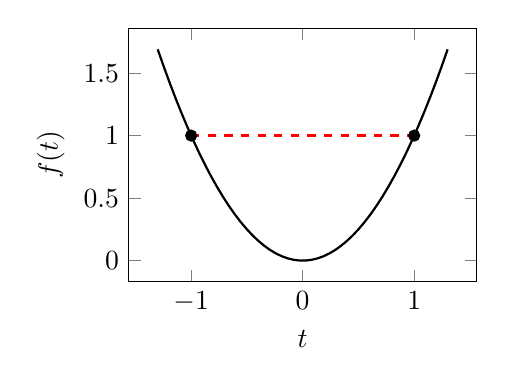
\begin{tikzpicture}
\begin{axis}[width=6cm,height=4.8cm,xlabel={$t$},ylabel={$f(t)$}]
\addplot[domain=-1.3:1.3,samples=50,thick] {x^2};
\addplot[dashed,thick,red] coordinates {(-1,1) (1,1)};
\addplot[only marks,mark=*] coordinates {(-1,1) (1,1)};
\end{axis}
\end{tikzpicture}\quad
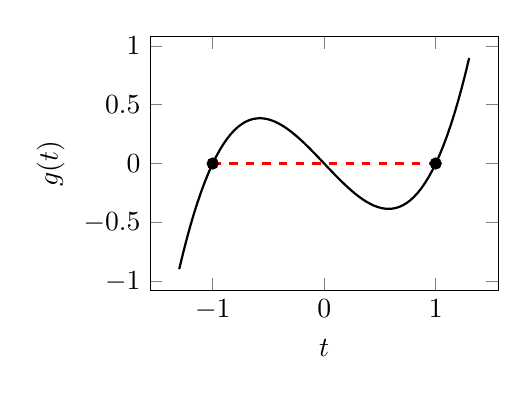
\begin{tikzpicture}
\begin{axis}[width=6cm,height=4.8cm,xlabel={$t$},ylabel={$g(t)$}]
\addplot[domain=-1.3:1.3,samples=80,thick] {x^3-x};
\addplot[dashed,thick,red] coordinates {(-1,0) (1,0)};
\addplot[only marks,mark=*] coordinates {(-1,0) (1,0)};
\end{axis}
\end{tikzpicture}
\caption{The chord between two points of the graph. Left: $f(t)=t^{2}$, the chord from
$(-1,1)$ to $(1,1)$ has value $1$ at $t=0$ whereas the graph has $0$, so the chord lies above
the graph. Right: $g(t)=t^{3}-t$, the chord from $(-1,0)$ to $(1,0)$ crosses the graph at
$t=-1$, $0$, $1$; at $t=-0.5$ the graph has value $0.375$ whereas the chord has $0$.}
\label{fig:fungsi-konveks}
\end{figure}

That definition is equivalent to a geometric statement about the \emph{epigraph}, that is the
set of points above the graph: $f$ is convex exactly when
$\operatorname{epi}f=\{(\mathbf{x},t):f(\mathbf{x})\le t\}$ is convex. The equivalence is
purely algebraic, and it turns a question about functions into a question about sets.

For differentiable functions there are two far faster tests, and both are
necessary-and-sufficient, not merely sufficient.

\begin{teorema}[First-order test]
Let $f$ be differentiable on an open convex set $C$. The function $f$ is convex if and only
if
\[
  f(\mathbf{y})\ge f(\mathbf{x})+\nabla f(\mathbf{x})^{\top}(\mathbf{y}-\mathbf{x})
\]
for all $\mathbf{x},\mathbf{y}\in C$.
\end{teorema}

\begin{proof}
Suppose $f$ is convex, take $\mathbf{x}\ne\mathbf{y}$ and $t\in(0,1)$. From the definition,
\[
  \frac{f\bigl(\mathbf{x}+t(\mathbf{y}-\mathbf{x})\bigr)-f(\mathbf{x})}{t}
  \le f(\mathbf{y})-f(\mathbf{x}).
\]
As $t\downarrow0$ the left side tends to the directional derivative
$\nabla f(\mathbf{x})^{\top}(\mathbf{y}-\mathbf{x})$, so the required inequality holds in the
limit. For the converse direction, suppose that inequality holds and take
$\mathbf{z}=t\mathbf{x}+(1-t)\mathbf{y}$ with $t\in[0,1]$. Apply the inequality at
$\mathbf{z}$ against $\mathbf{x}$ and against $\mathbf{y}$:
\[
  f(\mathbf{x})\ge f(\mathbf{z})+\nabla f(\mathbf{z})^{\top}(\mathbf{x}-\mathbf{z}),
  \qquad
  f(\mathbf{y})\ge f(\mathbf{z})+\nabla f(\mathbf{z})^{\top}(\mathbf{y}-\mathbf{z}).
\]
Multiply the first by $t$, the second by $1-t$, then add. The gradient terms vanish because
$t(\mathbf{x}-\mathbf{z})+(1-t)(\mathbf{y}-\mathbf{z})=\mathbf{0}$, and what remains is
$t\,f(\mathbf{x})+(1-t)f(\mathbf{y})\ge f(\mathbf{z})$.
\end{proof}

The practical reading: the graph lies above every tangent plane. A single tangent plane
already gives a global lower bound, and that is why the gradient at any point becomes an
honest tool rather than a local forecast.

\begin{teorema}[Second-order test]
Let $f$ be twice differentiable on an open convex set $C$. The function $f$ is convex if and
only if the Hessian $\nabla^{2}f(\mathbf{x})$ is positive semidefinite for every
$\mathbf{x}\in C$, that is
$\mathbf{v}^{\top}\nabla^{2}f(\mathbf{x})\mathbf{v}\ge0$ for all $\mathbf{v}$.
\index{Hessian}
\end{teorema}

\begin{proof}
If $f$ is convex, then for every $\mathbf{x}$ and $\mathbf{v}$ the one-variable function
$g(s)=f(\mathbf{x}+s\mathbf{v})$ is convex on an interval around zero, because composition
with an affine map preserves convexity. The first-order test on $g$ shows that $g'$ is
increasing, so $g''(0)\ge0$; and $g''(0)=\mathbf{v}^{\top}\nabla^{2}f(\mathbf{x})
\mathbf{v}$.

Conversely, if the Hessian is positive semidefinite on all of $C$, Taylor's theorem with
integral remainder (Chapter 12) gives
\[
  f(\mathbf{y})=f(\mathbf{x})+\nabla f(\mathbf{x})^{\top}(\mathbf{y}-\mathbf{x})
  +\int_{0}^{1}(1-s)\,(\mathbf{y}-\mathbf{x})^{\top}
   \nabla^{2}f\bigl(\mathbf{x}+s(\mathbf{y}-\mathbf{x})\bigr)(\mathbf{y}-\mathbf{x})\,ds .
\]
The integrand is nonnegative because the Hessian is positive semidefinite and $(1-s)\ge0$, so
the integral term is nonnegative. The first-order inequality holds, and $f$ is convex.
\end{proof}

Two warnings about the second-order test. First, a Hessian that is positive
\emph{definite} suffices for strict convexity, but is not a necessary condition:
$f(x)=x^{4}$ is strictly convex although $f''(0)=0$. Second, a positive semidefinite Hessian
gives convexity only, not strictness; $f(x_{1},x_{2})=x_{1}^{2}$ has Hessian
$\operatorname{diag}(2,0)$ and its minimum is the entire line $x_{1}=0$.

\begin{bacakeras}
Two voices, read alternately with a friend. The first voice asks, the second answers.

``I drop a marble into the bowl. Where does it go?'' ``To the bottom. Always to the same
bottom.'' ``And if I release it from the other side?'' ``To that bottom too.'' ``So there is
only one lowest place?'' ``Only one, and every descending path finds it.''

``Now I release it on a stone slope. Where does it go?'' ``Into the first hollow that is deep
enough.'' ``Is that the deepest one?'' ``Not necessarily. That hollow holds it, it does not
convince it.''

Repeat alternately, faster and faster, with drumming on the table: a bowl has no traps, a
hillside has traps.

The line the reader must repeat, once, in a clear voice: if every descending path ends at the
same point, there are no traps there, and that is what convex means.
\end{bacakeras}

Several operations preserve convexity. The sum of two convex functions stays convex, because
the inequalities are added; a positive multiple does too. The composition
$f(\mathbf{A}\mathbf{x}+\mathbf{b})$ is convex when $f$ is convex, because an affine map
sends mixtures to mixtures. The pointwise maximum is convex as well: if $f=\max_{i}f_{i}$,
the inequality for each $f_{i}$ holds for the maximum. That explains why
$\max\{|x_{1}|,|x_{2}|\}$ has a crease and is still convex.

\begin{resep}
Four steps to check convexity, from the cheapest.
\begin{enumerate}
  \item Check the region first: take two points in $C$ and make sure the segment between them
        stays in $C$. If that fails, stop, because the next tests assume that $C$ is convex.
  \item Test through the definition with a general pair $\mathbf{x},\mathbf{y}$: write
        $f(t\mathbf{x}+(1-t)\mathbf{y})$ and compare it with
        $t\,f(\mathbf{x})+(1-t)f(\mathbf{y})$ for $t\in[0,1]$. One pair that reverses the
        inequality is enough to reject.
  \item Compute the Hessian $\nabla^{2}f(\mathbf{x})$ as a function of $\mathbf{x}$, not as
        one matrix of numbers at one point.
  \item Decide the sign: nonnegative eigenvalues, or all leading principal minors from
        $1\times1$ up to $n\times n$ nonnegative. One negative eigenvalue closes the case.
\end{enumerate}
A warning about the order: step 4 must not be taken before step 1. A Hessian that is positive
definite at one point speaks only about that point, whereas the definition speaks about all of
$C$.
\end{resep}

\section{Standard form and why a local optimum becomes global}
\tingkat{intermediate}

Up to here we have two separate ideas: a region with no holes and a surface that does not bend
upward. Optimization unites the two through a single way of writing. Every optimization
problem can be written in the same way: one function to be made small, a set of inequality
conditions, and a set of equality conditions.

\kamus{standard form}{bentuk baku}{A way of writing every optimization problem with one
pattern: one objective, conditions of the form ``no more than zero'', and conditions of the
form ``equals''.}

\begin{definisi}[Optimization problem in standard form]
An \emph{optimization problem in standard form} is
\[
  \begin{array}{ll}
  \text{minimize} & f_{0}(\mathbf{x})\\
  \text{subject to} & f_{i}(\mathbf{x})\le0,\qquad i=1,\dots,m,\\
                & h_{j}(\mathbf{x})=0,\qquad j=1,\dots,p,
  \end{array}
\]
with variable $\mathbf{x}\in\mathbb{R}^{n}$, objective function $f_{0}$, inequality constraint
functions $f_{i}$, and equality constraint functions $h_{j}$. Its domain is
$D=\bigcap_{i}\operatorname{dom}f_{i}\cap\bigcap_{j}\operatorname{dom}h_{j}$, its feasible
region is $X=\{\mathbf{x}\in D:f_{i}(\mathbf{x})\le0,\ h_{j}(\mathbf{x})=0\}$, and the
\emph{optimal value} is $p^{*}=\inf_{\mathbf{x}\in X}f_{0}(\mathbf{x})$, possibly $-\infty$
when the problem is unbounded below. The problem is called a \emph{convex problem} when
$f_{0},\dots,f_{m}$ are convex and $h_{1},\dots,h_{p}$ are affine.
\index{standard form}
\end{definisi}

That every constraint can be brought to this pattern is easy to check. The condition
$f(\mathbf{x})\ge b$ becomes $b-f(\mathbf{x})\le0$; a linear equality stays an equality;
maximizing $f$ is the same as minimizing $-f$. What is not free is convexity alone: flipping
the sign of an inequality flips the convexity of the function, so the direction of an
inequality must not be changed without checking again.

\begin{akibat}[Convex feasible region]
In a convex problem, the feasible region $X$ is convex.
\end{akibat}

\begin{proof}
The sublevel set $S_{i}=\{\mathbf{x}:f_{i}(\mathbf{x})\le0\}$ is convex for every $i$: if
$f_{i}(\mathbf{x})\le0$ and $f_{i}(\mathbf{y})\le0$, convexity gives
$f_{i}(t\mathbf{x}+(1-t)\mathbf{y})\le t\,f_{i}(\mathbf{x})+(1-t)f_{i}(\mathbf{y})\le0$.
The set $\{\mathbf{x}:h_{j}(\mathbf{x})=0\}$ is a hyperplane because $h_{j}$ is affine, hence
convex. The feasible region is the intersection of all of them, and an intersection of convex
sets is convex by the proposition in the first section.
\end{proof}

That corollary is what makes this whole chapter make sense: two feasible points can always be
joined without leaving the feasible region. The simplest polyhedron is the feasible region of a
two-variable linear program in Figure~\ref{fig:lp-verteks}: a quadrilateral, and its linear
objective is optimal at a vertex.

\begin{figure}[!ht]
\centering
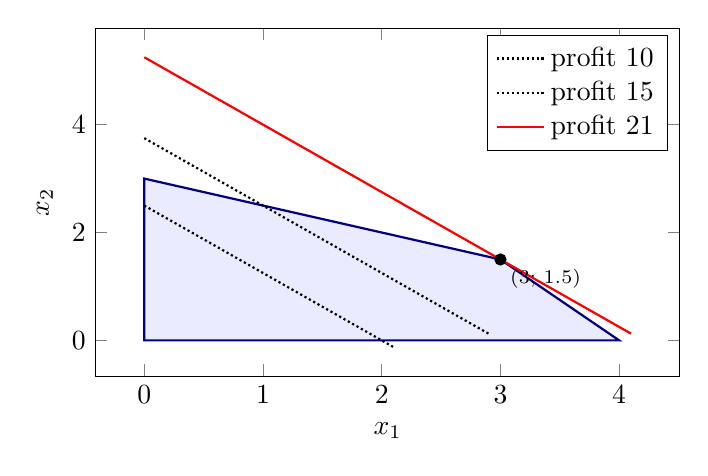
\begin{tikzpicture}
\begin{axis}[width=9cm,height=6cm,xlabel={$x_{1}$},ylabel={$x_{2}$}]
\addplot[forget plot,fill=blue!8,draw=blue!50!black,thick]
  coordinates {(0,0) (4,0) (3,1.5) (0,3)} \closedcycle;
\addplot[domain=0:2.1,densely dotted,thick] {2.5-1.25*x};
\addlegendentry{profit $10$}
\addplot[domain=0:2.9,densely dotted,thick] {3.75-1.25*x};
\addlegendentry{profit $15$}
\addplot[domain=0:4.1,thick,red] {5.25-1.25*x};
\addlegendentry{profit $21$}
\addplot[forget plot,only marks,mark=*] coordinates {(3,1.5)};
\node[font=\scriptsize,below right] at (axis cs:3,1.5) {$(3;\,1.5)$};
\end{axis}
\end{tikzpicture}
\caption{The feasible region of the workshop linear program of Chapter 24:
$6x_{1}+4x_{2}\le24$ (plywood), $x_{1}+2x_{2}\le6$ (hours), $x_{1},x_{2}\ge0$, objective
$5x_{1}+4x_{2}$. The vertices $(0;0)$, $(4;0)$, $(3;1.5)$, $(0;3)$ have values $0$, $20$,
$21$, $12$. The level line $21$ touches only the vertex $(3;1.5)$; the line $20$ still cuts
the feasible region.}
\label{fig:lp-verteks}
\end{figure}


Now the statement promised by the chapter opening, and its proof is short precisely because
the feasible region is convex.

\begin{teorema}[A local minimum is a global minimum]
Let $f_{0}$ be convex on a convex set $X$, and let $\mathbf{x}^{*}\in X$ satisfy
$f_{0}(\mathbf{x}^{*})\le f_{0}(\mathbf{x})$ for every $\mathbf{x}\in X$ close enough to
$\mathbf{x}^{*}$. Then $f_{0}(\mathbf{x}^{*})\le f_{0}(\mathbf{x})$ for every
$\mathbf{x}\in X$. The set of all minimum points is convex as well.
\index{global optimum}
\end{teorema}

\begin{proof}
Suppose there is $\mathbf{y}\in X$ with $f_{0}(\mathbf{y})<f_{0}(\mathbf{x}^{*})$. For
$t\in(0,1]$ the point $\mathbf{z}_{t}=(1-t)\mathbf{x}^{*}+t\mathbf{y}$ lies in $X$ and
concentrates at $\mathbf{x}^{*}$ as $t\to0$, so for $t$ small enough it enters the
neighborhood where $\mathbf{x}^{*}$ is a local minimum. But convexity gives
\[
  f_{0}(\mathbf{z}_{t})\le(1-t)f_{0}(\mathbf{x}^{*})+t\,f_{0}(\mathbf{y})
  <f_{0}(\mathbf{x}^{*}),
\]
contrary to local minimality. For the second part, if $\mathbf{x}^{*},\mathbf{y}^{*}$ are both
minimum with value $p^{*}$, then $f_{0}(\mathbf{z}_{t})\le p^{*}$, whereas $p^{*}$ is the
smallest possible value, so $f_{0}(\mathbf{z}_{t})=p^{*}$ and $\mathbf{z}_{t}$ is a minimum
too.
\end{proof}

\begin{akibat}[Stationary condition without constraints]
If $f$ is convex and differentiable on an open set, then
$\nabla f(\mathbf{x}^{*})=\mathbf{0}$ if and only if $\mathbf{x}^{*}$ is a global minimum.
\end{akibat}

\begin{proof}
If $\nabla f(\mathbf{x}^{*})=\mathbf{0}$, the first-order test gives
$f(\mathbf{y})\ge f(\mathbf{x}^{*})$ for every $\mathbf{y}$. Conversely, if
$\mathbf{x}^{*}$ is a minimum, then for every direction $\mathbf{v}$ and small $t>0$ we have
$f(\mathbf{x}^{*}+t\mathbf{v})\ge f(\mathbf{x}^{*})$, hence the directional derivative
$\nabla f(\mathbf{x}^{*})^{\top}\mathbf{v}\ge0$. Since $\mathbf{v}$ may also be replaced by
$-\mathbf{v}$, it must be that $\nabla f(\mathbf{x}^{*})=\mathbf{0}$.
\end{proof}

\begin{tangan}
Materials: two meters of string, one small ring, a blindfold, and a friend.

Tie the string between two posts of equal height, then stretch it straight. Ask the friend to
close their eyes, to hang the ring at the middle of the string, and to slide it slowly left and
right with one finger. The ring slides to the lowest point, wherever it is released. Ask the
friend to mark the stopping point without opening their eyes; repeat five times from different
starting positions. All the marks must fall on one point.

Now tie a small knot in the string, a little to the left, so that the string forms two
hollows. Repeat the experiment. The ring stops in the left hollow when released near there,
and in the middle when released to the right of the knot: two stopping places, two valleys.

What must be visible: a string without a knot has only one lowest point, a string with a knot
has two, and a finger that stops in the left hollow does not know what happens on the right,
exactly like an algorithm that stops at the first stationary point.
\end{tangan}

Without convexity, that corollary is false. Take $f(x_{1},x_{2})=x_{1}x_{2}$ on the square
$[-1,1]^{2}$. Its gradient $(x_{2},x_{1})$ vanishes at the origin, whereas
$f(\mathbf{0})=0$ while $f(1,-1)=-1$. Its Hessian is
$\begin{pmatrix}0&1\\1&0\end{pmatrix}$ with eigenvalues $1$ and $-1$, so the second-order test
rejects convexity: the origin is a saddle, not a valley. Chapter 24 gives a more deceptive
example: rounding a continuous answer gives a profit of 19, whereas the best integer answer
gives 20.

\section{The Lagrangian and lower bounds from the dual}
\tingkat{advanced}

A constraint always has the form ``something must not be positive'', so we can put a price on
violating it: every time $f_{i}(\mathbf{x})$ is positive we pay a fine $\lambda_{i}$ per
unit, and every deviation $h_{j}(\mathbf{x})$ from zero is paid or received at $\nu_{j}$ per
unit. The resulting function is no larger than the original objective, provided the price is
nonnegative. A bad price gives a loose bound; a good price gives an exact bound.

\begin{definisi}[Lagrangian and dual function]
For a problem in standard form, its \emph{Lagrangian} is
\[
  L(\mathbf{x},\boldsymbol{\lambda},\boldsymbol{\nu})
  =f_{0}(\mathbf{x})+\sum_{i=1}^{m}\lambda_{i}f_{i}(\mathbf{x})
   +\sum_{j=1}^{p}\nu_{j}h_{j}(\mathbf{x}),
\]
with $\boldsymbol{\lambda}\in\mathbb{R}^{m}$ and $\boldsymbol{\nu}\in\mathbb{R}^{p}$ called
\emph{multipliers} or \emph{dual variables}. The \emph{dual function} is its infimum over the
original variable,
\[
  g(\boldsymbol{\lambda},\boldsymbol{\nu})
  =\inf_{\mathbf{x}\in D}L(\mathbf{x},\boldsymbol{\lambda},\boldsymbol{\nu}),
\]
and the \emph{dual problem} is to maximize $g$ under the condition
$\boldsymbol{\lambda}\ge\mathbf{0}$. A pair $(\boldsymbol{\lambda},\boldsymbol{\nu})$ is
called \emph{dual feasible} when $\boldsymbol{\lambda}\ge\mathbf{0}$ and
$g(\boldsymbol{\lambda},\boldsymbol{\nu})>-\infty$. Its optimal value is written $d^{*}$.
\index{Lagrangian}\index{duality}
\end{definisi}

\begin{proposisi}[The dual function is always concave]
$g$ is the infimum of affine functions in $(\boldsymbol{\lambda},\boldsymbol{\nu})$, because
for every fixed $\mathbf{x}$ the function $L(\mathbf{x},\cdot,\cdot)$ is affine. Hence $g$ is
concave, and the dual problem is always a convex problem, whatever the shape of the original
problem.
\end{proposisi}

\begin{proof}
Take two dual points $(\boldsymbol{\lambda},\boldsymbol{\nu})$ and
$(\boldsymbol{\lambda}',\boldsymbol{\nu}')$ and $t\in[0,1]$. For every $\mathbf{x}$,
linearity gives
\[
  L\bigl(\mathbf{x},\,t\boldsymbol{\lambda}+(1-t)\boldsymbol{\lambda}',\,
  t\boldsymbol{\nu}+(1-t)\boldsymbol{\nu}'\bigr)
  =t\,L(\mathbf{x},\boldsymbol{\lambda},\boldsymbol{\nu})
   +(1-t)\,L(\mathbf{x},\boldsymbol{\lambda}',\boldsymbol{\nu}').
\]
Take the infimum of both sides over $\mathbf{x}$; the infimum of a sum is no less than the sum
of the infima, so
$g\ge t\,g(\boldsymbol{\lambda},\boldsymbol{\nu})
+(1-t)g(\boldsymbol{\lambda}',\boldsymbol{\nu}')$, that is $g$ is concave.
\end{proof}

A pleasant corollary: maximizing a concave function under the constraint
$\boldsymbol{\lambda}\ge\mathbf{0}$ is always a convex problem. Every problem, even one full of
holes, has a convex twin; the twin does not always give the same answer, but it always gives a
bound.

\begin{teorema}[Weak duality]
For every dual feasible $(\boldsymbol{\lambda},\boldsymbol{\nu})$ and every primal feasible
$\mathbf{x}$ we have $L(\mathbf{x},\boldsymbol{\lambda},\boldsymbol{\nu})\le
f_{0}(\mathbf{x})$. Hence $g(\boldsymbol{\lambda},\boldsymbol{\nu})\le p^{*}$, that is
$d^{*}\le p^{*}$.
\end{teorema}

\begin{proof}
Take $\mathbf{x}\in X$. Every $f_{i}(\mathbf{x})\le0$ and $\lambda_{i}\ge0$, so
$\lambda_{i}f_{i}(\mathbf{x})\le0$. Every $h_{j}(\mathbf{x})=0$, so
$\nu_{j}h_{j}(\mathbf{x})=0$ whatever $\nu_{j}$ is. Therefore
$L(\mathbf{x},\boldsymbol{\lambda},\boldsymbol{\nu})\le f_{0}(\mathbf{x})$. That inequality
holds for every feasible $\mathbf{x}$, hence also for the infimum over all feasible
$\mathbf{x}$; the infimum over all of $D$ is no larger, so
$g(\boldsymbol{\lambda},\boldsymbol{\nu})\le p^{*}$. The last inequality is taken over all
dual feasible pairs.
\end{proof}

That proof uses neither convexity nor differentiability, so weak duality holds for integer
problems, combinatorial problems, and any problem at all in standard form. That is why dual
lower bounds are used in branch and bound in Chapter 24: the bound is valid even though the
relaxation is not the answer.

The difference $p^{*}-d^{*}$ is called the \emph{duality gap}. Since
$d^{*}\le p^{*}$, the gap is never negative. When the gap is zero, we say that
\emph{strong duality} holds; the next section discusses when that happens.
\index{weak duality}\index{duality gap}

Before that, one corollary used to check computed results. If there is a feasible point
$\mathbf{x}$ and a dual feasible pair $(\boldsymbol{\lambda},\boldsymbol{\nu})$ with
$f_{0}(\mathbf{x})=g(\boldsymbol{\lambda},\boldsymbol{\nu})$, then
$d^{*}\ge g=f_{0}(\mathbf{x})\ge p^{*}\ge d^{*}$, so all the inequalities become equalities:
the point is optimal, the pair is optimal, and the gap is zero. Equality of values is a
certificate of optimality that can be checked without knowing the answer in advance.

\begin{untukanak}
Have you ever haggled in a market? You name one price, the seller names another, and if the
bargaining stops halfway, neither of you knows the true price yet. But you already know one
thing: the seller will not go below a certain number, and you will not go above a certain
number. Those two numbers cage the true price, even though nobody has ever spoken it.

The idea of duality works exactly like that. Instead of looking for the answer, we attach a
price to each demand, then ask: with this price list, what is the worst outcome still possible?
Every sensible price list gives one number that the true answer cannot exceed. If some price
list gives a number equal to the answer we found, the matter is settled.

In this chapter we shall learn why such a price list always exists, why it sometimes fails to
close the gap, and why the gap that remains can be measured by a number.
\end{untukanak}

\section{Strong duality and Slater's condition}
\tingkat{advanced}

Convexity turns a local minimum into a global one, but it does not yet guarantee a zero
duality gap. What is missing is a condition about the \emph{geometry of feasibility}: if the
feasible region only touches the boundary of a constraint without entering it, there is no
sufficiently clean separating plane. That condition is named after Slater.

\begin{teorema}[Slater's condition]
Let the problem be convex, $f_{0},\dots,f_{m}$ differentiable, and
$h_{j}(\mathbf{x})=\mathbf{a}_{j}^{\top}\mathbf{x}-b_{j}$. If there is a feasible point
$\mathbf{x}\in\operatorname{ri}D$ with $f_{i}(\mathbf{x})<0$ for every $i$ and
$h_{j}(\mathbf{x})=0$ for every $j$, then strong duality holds, $d^{*}=p^{*}$, and the optimal
value of the dual is attained. If some of the inequality constraints turn out to be affine,
only the constraints that are not affine need be satisfied strictly.
\index{Slater}
\end{teorema}

A point with $f_{i}(\mathbf{x})<0$ is called \emph{strictly feasible}. The existence of one such
point is enough, and the condition demands nothing about the objective function.

The proof is not carried out here. The route is this: the set
$\mathcal{A}=\{(u,t):\exists\mathbf{x},\ f_{i}(\mathbf{x})\le u_{i},\
h_{j}(\mathbf{x})=0,\ f_{0}(\mathbf{x})\le t\}$ is convex, and the point $(0,p^{*})$ lies on
its boundary; the hyperplane separation theorem (Chapter 10 uses a similar idea for projection)
gives a supporting plane with coefficients $(\boldsymbol{\lambda},\boldsymbol{\nu})$ and value
$d^{*}$. The full proof is in Boyd and Vandenberghe section 5.3.2, and that theorem is what
justifies the step ``solve KKT and then trust the result''.

Slater is sufficient, not necessary, and the difference shows in the following small example.
Take $\min x$ with constraint $x^{2}\le0$. Its feasible region is a single point, $x=0$, so
there is no strictly feasible point and Slater fails. Its optimal value is $p^{*}=0$. The
Lagrangian $L=x+\lambda x^{2}$ gives $g(\lambda)=-1/(4\lambda)$ for $\lambda>0$, because the
minimum occurs at $x=-1/(2\lambda)$, so $\sup_{\lambda\ge0}g(\lambda)=0=d^{*}$. Strong duality
still holds, but that value is only approached, not attained: at every finite $\lambda$,
$g(\lambda)<0$. So what is lost when Slater fails is not always equality of values, but the
guarantee that the dual optimum is attained.

Conversely, Slater guarantees something that strong duality alone does not give: optimal
multipliers exist, so that the KKT equations have a solution to look for.

\section{The KKT conditions: necessary, and sufficient when convex}
\tingkat{advanced}

If the multipliers are already optimal, the optimal primal point must minimize the Lagrangian
without constraints, and there the gradient vanishes. Expanding that condition component by
component gives four groups of equations: the Karush-Kuhn-Tucker conditions.

\kamus{Lagrange multiplier}{pengali Lagrange}{The price per unit of violating a constraint; zero
means that constraint is not pressing, positive means that it is pressing.}

\begin{definisi}[KKT conditions]
A point $(\mathbf{x},\boldsymbol{\lambda},\boldsymbol{\nu})$ satisfies the \emph{KKT
conditions} when
\[
  \begin{array}{ll}
  f_{i}(\mathbf{x})\le0,\quad h_{j}(\mathbf{x})=0, & \text{(primal feasibility)}\\
  \lambda_{i}\ge0, & \text{(dual feasibility)}\\
  \lambda_{i}f_{i}(\mathbf{x})=0,\quad i=1,\dots,m, & \text{(complementary slackness)}\\
  \nabla f_{0}(\mathbf{x})+\sum_{i}\lambda_{i}\nabla f_{i}(\mathbf{x})
  +\sum_{j}\nu_{j}\nabla h_{j}(\mathbf{x})=\mathbf{0}. & \text{(stationarity)}
  \end{array}
\]
\index{KKT}\index{Lagrange multiplier}\index{complementary slackness}
\end{definisi}

The third group causes the most misunderstanding, so let us translate it: a multiplier may be
nonzero only for a constraint that is really pressing. A loose constraint is paid nothing,
because loosening it changes nothing. A zero multiplier on a pressing constraint is also
possible, and that is a sign of degeneracy.

The geometric side of the last group is visible in Figure~\ref{fig:kkt-singgung}.

\begin{figure}[!ht]
\centering
\begin{tikzpicture}[scale=1.42]
  \draw[->,layergrey] (-0.3,0)--(4.4,0) node[right,font=\small]{$x_{1}$};
  \draw[->,layergrey] (0,-0.3)--(0,4.4) node[above,font=\small]{$x_{2}$};
  \fill[layerteal!10] (0,0) circle (2);
  \begin{scope}
    \clip (-0.3,-0.3) rectangle (4.3,4.3);
    \draw[layergrey,densely dashed] (2.6,2.6) circle (1.25);
    \draw[layergrey,densely dashed] (2.6,2.6) circle (2.15);
    \draw[thick,accent] (2.6,2.6) circle (1.677);
  \end{scope}
  \draw[very thick,layerteal] (0,0) circle (2);
  \node[font=\scriptsize,layerteal,fill=white,inner sep=1pt,anchor=west]
    at (-0.4,1.9) {$f_{1}(\mathbf{x})=0$};
  \node[font=\scriptsize,accent,fill=white,inner sep=1pt,anchor=south east]
    at (1.1,2.02) {$f_{0}=2.81$};
  \node[font=\scriptsize,layergrey,fill=white,inner sep=1pt]
    at (2.6,3.9) {smaller value, not feasible};
  \fill[layergrey] (2.6,2.6) circle (1.4pt);
  \node[font=\scriptsize,layergrey,anchor=west] at (2.72,2.6) {$\mathbf{c}$};
  \fill[accent] (1.414,1.414) circle (1.9pt);
  \node[font=\scriptsize,accent,below left=-2pt] at (1.414,1.414)
    {$\mathbf{x}^{*}$};
  \draw[-{Latex},very thick,accent] (1.414,1.414)--(0.8,0.8)
    node[below right=-1pt,font=\scriptsize]{$\nabla f_{0}$};
  \draw[-{Latex},very thick,layerteal] (1.414,1.414)--(2.03,2.03)
    node[above left=-1pt,font=\scriptsize]{$\lambda\nabla f_{1}$};
\end{tikzpicture}
\caption{The contours of the objective $f_{0}(\mathbf{x})=(x_{1}-2.6)^{2}+(x_{2}-2.6)^{2}$,
concentric around the point $\mathbf{c}=(2.6;\,2.6)$, which is the unconstrained minimum and
falls outside the feasible region
$f_{1}(\mathbf{x})=x_{1}^{2}+x_{2}^{2}-4\le0$. The contour $f_{0}=2.81$ only touches the
constraint circle at $\mathbf{x}^{*}=(\sqrt{2};\sqrt{2})$; the deeper dashed contours have
smaller values but lie entirely outside the feasible region, whereas the outer ones still cut
the feasible region with larger values. At that point of tangency $\nabla f_{0}$ and
$\nabla f_{1}$ are parallel and oppositely directed, with a positive multiplier.}
\label{fig:kkt-singgung}
\end{figure}

Now the statement that gives this section its title, and which must be read carefully because
its two directions have different conditions.

\begin{teorema}[KKT is sufficient for optimality]
Let the problem be convex, $f_{0},\dots,f_{m}$ differentiable, and $h_{j}$ affine. If
$(\mathbf{x},\boldsymbol{\lambda},\boldsymbol{\nu})$ satisfies the KKT conditions, then
$\mathbf{x}$ is primal optimal, $(\boldsymbol{\lambda},\boldsymbol{\nu})$ is dual optimal, and
the duality gap is zero.
\end{teorema}

\begin{proof}
Because $\lambda_{i}\ge0$ and $f_{i}$ is convex, every term $\lambda_{i}f_{i}$ is convex;
because $h_{j}$ is affine, every term $\nu_{j}h_{j}$ is affine. So
$L(\cdot,\boldsymbol{\lambda},\boldsymbol{\nu})$ is convex in $\mathbf{x}$. The stationarity
condition says that its gradient vanishes at $\mathbf{x}$, so by the corollary in the third
section that point minimizes $L$ globally:
$g(\boldsymbol{\lambda},\boldsymbol{\nu})=L(\mathbf{x},\boldsymbol{\lambda},
\boldsymbol{\nu})$. Primal feasibility and complementary slackness remove all the constraint
terms:
\[
  g(\boldsymbol{\lambda},\boldsymbol{\nu})
  =f_{0}(\mathbf{x})+\sum_{i}\lambda_{i}f_{i}(\mathbf{x})
   +\sum_{j}\nu_{j}h_{j}(\mathbf{x})=f_{0}(\mathbf{x}).
\]
Because $g\le d^{*}\le p^{*}\le f_{0}(\mathbf{x})$ by weak duality, all those inequalities
become equalities. Hence $\mathbf{x}$ is primal optimal, the pair is dual optimal, and
$p^{*}-d^{*}=0$.
\end{proof}

The opposite direction is different in nature, and the difference is not technical.

\begin{teorema}[KKT is necessary under a qualification condition]
Let the problem be convex and differentiable, satisfy Slater's condition, and let
$\mathbf{x}^{*}$ be primal optimal with $p^{*}$ finite. Then there exists
$(\boldsymbol{\lambda}^{*},\boldsymbol{\nu}^{*})$ such that
$(\mathbf{x}^{*},\boldsymbol{\lambda}^{*},\boldsymbol{\nu}^{*})$ satisfies the KKT conditions.
\end{teorema}

The proof uses the hyperplane separation theorem on the achievable set, and is not repeated
here; see Boyd and Vandenberghe section 5.5.3. What must be remembered is the role of Slater in
it: without a qualification condition, an optimal point may fail KKT altogether, so that
``solve KKT'' is not a legitimate route for finding the answer.

The smallest counterexample is $\min x$ with constraint $x^{2}\le0$. Its optimal point is
$x^{*}=0$ and $\nabla f_{0}=1$, whereas $\nabla f_{1}=2x=0$ at that point. Stationarity demands
$1+\lambda\cdot0=0$, which is impossible. So that optimal point does not satisfy KKT, and what
fails is only the constraint qualification: the feasible region is one point, there is no
direction to move, there is no supporting plane.

The logical conclusion, and it is often quoted wrongly: in a convex problem, KKT is
\emph{sufficient} without extra conditions, but \emph{necessary} only when a constraint
qualification is present. The statement ``$\mathbf{x}$ is optimal if and only if there are
multipliers satisfying KKT'' demands both directions, so Slater is part of it.

One interpretation for remembering the multipliers. Suppose constraint $i$ is relaxed to
$f_{i}(\mathbf{x})\le u_{i}$, and the optimal value becomes $p^{*}(u)$. If $p^{*}$ is
differentiable at $u=0$, then
\[
  \lambda_{i}^{*}=-\frac{\partial p^{*}}{\partial u_{i}}(0).
\]
The multiplier is a shadow price: how much the objective value falls when that constraint is
relaxed by one unit. In the worked example later, relaxing the solubility limit from one half
to $0.6$ lowers the deviation from $2.5$ to $2.32$, whereas the shadow price predicts
$2.5-2(0.1)=2.30$. The difference $0.02$ is a second-order term, and its direction is always
the same: the linear forecast is a lower bound, so the improvement it promises is never
exceeded.

The mechanical interpretation, already used by Lagrange himself: two blocks are connected by a
spring and must not pass through each other or through the wall. Potential energy is the
objective function; at equilibrium, stationarity is the balance of forces, and the multiplier
is the contact force of the wall. A contact force only pushes, never pulls, that is
$\lambda_{i}\ge0$; it appears only when there is contact, that is complementary slackness (Boyd
and Vandenberghe section 5.5.4).

\begin{catatan}[Subgradients]
If $f$ is convex but not differentiable, the gradient is replaced by a \emph{subgradient}:
$\mathbf{s}$ is a subgradient of $f$ at $\mathbf{x}$ when
$f(\mathbf{y})\ge f(\mathbf{x})+\mathbf{s}^{\top}(\mathbf{y}-\mathbf{x})$ for every
$\mathbf{y}$; the set of all subgradients is written $\partial f(\mathbf{x})$. For
$f(x)=|x|$ at $x=0$ that set is the interval $[-1,1]$, because every slope between $-1$ and
$1$ gives a line below the graph. The optimality condition without constraints becomes
$\mathbf{0}\in\partial f(\mathbf{x}^{*})$, and KKT still holds with $\nabla f_{i}$ replaced by
a subgradient (Rockafellar section 23).\index{subgradient}
\end{catatan}

\section{Worked examples}
\tingkat{intermediate}

The following three computations are carried out to the last digit, with simple fractions so
that they can be checked by hand.

\emph{First, a convexity test through eigenvalues.} Take
$f(x_{1},x_{2})=x_{1}^{2}+4x_{1}x_{2}+5x_{2}^{2}$. Its Hessian is constant,
\[
  \nabla^{2}f=\begin{pmatrix}2&4\\4&10\end{pmatrix},
  \qquad
  \operatorname{tr}=12,\quad \det=20-16=4 .
\]
Its eigenvalues are $\lambda_{1,2}=6\pm\sqrt{36-4}=6\pm4\sqrt{2}$, that is $0.343146$ and
$11.656854$. Both are positive, so the Hessian is positive definite and $f$ is strictly convex.
For comparison, $g(x_{1},x_{2})=x_{1}^{2}-x_{2}^{2}$ has Hessian
$\operatorname{diag}(2,-2)$ with eigenvalues $2$ and $-2$: not convex, and its critical point at
the origin is a saddle. The function $h(x_{1},x_{2})=x_{1}^{2}$ has eigenvalues $0$ and $2$:
convex, not strict, and its minimum is the entire line $x_{1}=0$, so the answer is not unique.

\begin{tantangan}
Take $f(x_{1},x_{2})=x_{1}^{2}x_{2}^{2}$. Hold $x_{2}=c$ fixed: the graph is a parabola opening
upward, so every horizontal slice looks convex, and the same holds for every vertical slice. Is
$f$ convex on $\mathbb{R}^{2}$? If not, exhibit two points that prove it, then explain why
checking slice by slice is never enough.

Hint 1: do not move parallel to an axis. Move both coordinates at once, then check the midpoint.

Hint 2: compute $f(1,0)$, $f(0,1)$, and the value of $f$ at the midpoint of that segment; or
compute $\det\nabla^{2}f$ at $(1,1)$, which equals $-12x_{1}^{2}x_{2}^{2}$.

If you get stuck, go back to the section Convex functions and their two tests.
\end{tantangan}

\emph{Second, the paint mixer problem through KKT.} With $x_{1},x_{2}$ the amounts of the two
pigments, the problem is
\[
  \text{minimize } (x_{1}-2)^{2}+(x_{2}-2)^{2}
  \quad\text{subject to}\quad x_{1}+x_{2}=2,\quad x_{1}\le\tfrac12 .
\]
Write $g(\mathbf{x})=x_{1}-\tfrac12\le0$ and $h(\mathbf{x})=x_{1}+x_{2}-2=0$. Stationarity gives
\[
  2(x_{1}-2)+\lambda+\nu=0,\qquad 2(x_{2}-2)+\nu=0 ,
\]
and complementary slackness gives $\lambda(x_{1}-\tfrac12)=0$. If $\lambda=0$, the two
equations give $x_{1}=x_{2}$, and with $x_{1}+x_{2}=2$ we obtain $x_{1}=x_{2}=1$, which
violates $x_{1}\le\tfrac12$. So $\lambda>0$: $x_{1}=\tfrac12$ and $x_{2}=\tfrac32$. The second
equation gives $\nu=2(2-\tfrac32)=1$, the first gives
$\lambda=4-2x_{1}-\nu=4-1-1=2$. Since $\lambda=2\ge0$, that point is globally optimal by the
sufficiency theorem, with
\[
  p^{*}=\bigl(\tfrac12-2\bigr)^{2}+\bigl(\tfrac32-2\bigr)^{2}
  =\tfrac94+\tfrac14=\tfrac52=2.5 .
\]

Checking through the dual, not through trust. The dual function is computed by completing the
square in each variable:
\[
  \min_{x_{1}}\Bigl[(x_{1}-2)^{2}+(\lambda+\nu)x_{1}\Bigr]
  =4-\frac{(\lambda+\nu-4)^{2}}{4},
  \qquad
  \min_{x_{2}}\Bigl[(x_{2}-2)^{2}+\nu x_{2}\Bigr]
  =4-\frac{(\nu-4)^{2}}{4},
\]
so that
\[
  g(\lambda,\nu)=8-\frac{(\lambda+\nu-4)^{2}}{4}-\frac{(\nu-4)^{2}}{4}
  -\frac{\lambda}{2}-2\nu .
\]
At $(\lambda,\nu)=(2,1)$ we get $g=8-\tfrac14-\tfrac94-1-2=\tfrac52=p^{*}$: the gap is zero, as
the strong duality guaranteed by Slater requires, because $(0.4;\,1.6)$ is strictly feasible.
The partial derivatives give $-\tfrac12(\lambda+\nu-4)-\tfrac12(\nu-4)-2=0$ and
$-\tfrac12(\lambda+\nu-4)-\tfrac12=0$; from the second $\lambda+\nu=3$, then $\nu=1$ and
$\lambda=2$. That pair is the only maximizer.

The shadow prices can be checked with numbers. If the solubility limit is relaxed to $0.6$, the
answer is $x_{1}=0.6$, $x_{2}=1.4$, and $p^{*}=1.96+0.36=2.32$. The linear forecast
$p^{*}-\lambda\cdot0.1=2.5-0.2=2.30$ is off by $0.02$, and $0.02=\tfrac12\cdot4\cdot(0.1)^{2}$
exactly, because the second derivative of $p^{*}$ with respect to that limit is $4$. If the
demanded sum is raised to $2.1$ with the limit unchanged, the answer is $x_{1}=\tfrac12$,
$x_{2}=1.6$, and $p^{*}=2.25+0.16=2.41$; the forecast $2.5-\nu\cdot0.1=2.40$ is off by
$0.01=\tfrac12\cdot2\cdot(0.1)^{2}$. Both prices are slopes that can be used to decide, with an
error that can be computed.

\emph{Third, the duality gap on a nonconvex problem.} Take one variable,
\[
  \text{minimize } (x-2)^{2}\quad\text{subject to}\quad x^{3}-x\le0 .
\]
That constraint is equivalent to $x(x-1)(x+1)\le0$, so the feasible region is
$(-\infty,-1]\cup[0,1]$: two separate pieces, not convex. On $[0,1]$ the objective decreases,
so its smallest value is $1$ at $x=1$. On $(-\infty,-1]$ the objective increases to the left
from $x=-1$, which has value $9$. So $p^{*}=1$, attained at $x=1$.

The dual side is very different. The Lagrangian is $L=(x-2)^{2}+\lambda(x^{3}-x)$. For
$\lambda>0$ the cubic term dominates as $x\to-\infty$ and carries a negative sign, so
$L\to-\infty$ and $g(\lambda)=-\infty$: there is no lower bound to collect. Only $\lambda=0$
leaves a finite value, and there $g(0)=\min_{x}(x-2)^{2}=0$ at $x=2$. Hence $d^{*}=0$ and
\[
  p^{*}-d^{*}=1-0=1 ,
\]
a gap of $100\%$ of the optimal value itself. The lower bound from the dual here is not a loose
bound but a bound in the wrong place: $x=2$ is the unconstrained answer, and the constraint is
what determines the answer.

The same example shows why convexity cannot be removed from the sufficiency theorem. Check the
point $x=-1$, which is feasible because $(-1)^{3}-(-1)=0$. There
$\nabla f_{0}=2(x-2)=-6$ and $\nabla g=3x^{2}-1=2$, so stationarity demands $-6+2\lambda=0$, that
is $\lambda=3$; complementary slackness holds because the constraint is active. So
$(x,\lambda)=(-1,3)$ satisfies all four groups of KKT conditions, even though
$f_{0}(-1)=9$ while $p^{*}=1$.

\kertas{Repeat the second computation with the limit $x_{1}\le1$. Before computing, decide
whether that constraint is still pressing, then check whether its multiplier is still $2$.
After that compute the optimal value and compare it with $2.5$. As an extra exercise, find the
value of the limit $c$ at which the constraint stops pressing, and explain why the multiplier
must be zero exactly at that $c$.}

\section{Computational lab}
\tingkat{advanced}

The two blocks below were run with Python 3.14.4, numpy 2.5.2, and scipy 1.18.0. The output is
copied verbatim.

\begin{lab}
\begin{verbatim}
import numpy as np
from scipy.optimize import minimize

np.set_printoptions(precision=8, suppress=True, linewidth=78)

# mixer problem: min (x1-2)^2+(x2-2)^2  s.t. x1+x2=2, x1<=0.5
f  = lambda x: (x[0]-2)**2 + (x[1]-2)**2
df = lambda x: np.array([2*(x[0]-2), 2*(x[1]-2)])
cons = [{"type": "eq",   "fun": lambda x: x[0]+x[1]-2,
         "jac": lambda x: np.array([1., 1.])},
        {"type": "ineq", "fun": lambda x: 0.5-x[0],
         "jac": lambda x: np.array([-1., 0.])}]
r = minimize(f, [0., 0.], jac=df, constraints=cons, method="SLSQP",
             options={"ftol": 1e-15, "maxiter": 500})
xs = r.x
print("x* =", xs, " f(x*) =", f(xs))
print("multipliers (scipy):", r.multipliers)

# multipliers from stationarity, using the active set {eq, ineq}
A = np.column_stack([[1., 0.], [1., 1.]])   # columns: grad g, grad h
lam, nu = np.linalg.solve(A, -df(xs))
print("lambda, nu =", lam, nu)

# KKT residuals
print("h(x*)          =", xs[0]+xs[1]-2)
print("g(x*)          =", 0.5-xs[0])
print("lambda*g(x*)   =", lam*(0.5-xs[0]))
print("||grad L||     =", np.linalg.norm(df(xs) + lam*np.array([1.,0.])
                                         + nu*np.array([1.,1.])))

# dual function and its maximization
g = lambda lam, nu: (8 - (lam+nu-4)**2/4 - (nu-4)**2/4
                     - 0.5*lam - 2*nu)
print("g(2,1)         =", g(2., 1.))
rd = minimize(lambda z: -g(z[0], z[1]), [0.5, 0.5], method="SLSQP",
              bounds=[(0, None), (None, None)], options={"ftol": 1e-15})
print("dual argmax    =", rd.x, " d* =", -rd.fun)
print("gap p*-d*      =", f(xs) + rd.fun)

# Hessian eigenvalue test
for name, H in [("x1^2+4x1x2+5x2^2", np.array([[2.,4.],[4.,10.]])),
                ("x1^2-x2^2",        np.array([[2.,0.],[0.,-2.]])),
                ("x1^2",             np.array([[2.,0.],[0.,0.]]))]:
    print(name, "eig =", np.linalg.eigvalsh(H))
\end{verbatim}
Actual output:
\begin{verbatim}
x* = [0.5 1.5]  f(x*) = 2.500000000000001
multipliers (scipy): [-1.  2.]
lambda, nu = 2.0000000000000027 0.9999999999999987
h(x*)          = 0.0
g(x*)          = 6.106226635438361e-16
lambda*g(x*)   = 1.2212453270876738e-15
||grad L||     = 0.0
g(2,1)         = 2.5
dual argmax    = [1.99999997 0.99999999]  d* = 2.499999999999999
gap p*-d*      = 1.7763568394002505e-15
x1^2+4x1x2+5x2^2 eig = [ 0.34314575 11.65685425]
x1^2-x2^2 eig = [-2.  2.]
x1^2 eig = [0. 2.]
\end{verbatim}
\end{lab}

\begin{lab}
\begin{verbatim}
import numpy as np
from scipy.optimize import minimize

# nonconvex: min (x-2)^2  s.t. x^3 - x <= 0
f3 = lambda x: (x[0]-2)**2
r3 = minimize(f3, [0.5], constraints=[{"type": "ineq",
              "fun": lambda x: -(x[0]**3 - x[0])}],
              method="SLSQP", options={"ftol": 1e-14, "maxiter": 500})
print("x* =", r3.x, " p* =", f3(r3.x))

# Lagrangian for several lambda, evaluated far to the left
for lam in (0.0, 1e-3, 1e-2, 0.1):
    L = lambda x: (x[0]-2)**2 + lam*(x[0]**3 - x[0])
    print(f"lam={lam:<6} L(-1e4)={L(np.array([-1e4])):.3e}",
          f" L(-1e6)={L(np.array([-1e6])):.3e}")

# points that satisfy KKT but are not the answer
for xv in (-1.0, 1.0, 0.0):
    f0p = 2*(xv-2); gp = 3*xv*xv - 1
    lam = -f0p/gp if gp != 0 else float("nan")
    print(f"x={xv:>4}  f0'={f0p:>5}  g'={gp:>4}  lam={lam:>6}"
          f"  f0={ (xv-2)**2 }  feasible={xv**3-xv <= 0}")
\end{verbatim}
Actual output:
\begin{verbatim}
x* = [1.]  p* = 0.999999999995369
lam=0.0    L(-1e4)=1.000e+08  L(-1e6)=1.000e+12
lam=0.001  L(-1e4)=-9.000e+08  L(-1e6)=-9.990e+14
lam=0.01   L(-1e4)=-9.900e+09  L(-1e6)=-9.999e+15
lam=0.1    L(-1e4)=-9.990e+10  L(-1e6)=-1.000e+17
x=-1.0  f0'= -6.0  g'= 2.0  lam=   3.0  f0=9.0  feasible=True
x= 1.0  f0'= -2.0  g'= 2.0  lam=   1.0  f0=1.0  feasible=True
x= 0.0  f0'= -4.0  g'=-1.0  lam=  -4.0  f0=4.0  feasible=True
\end{verbatim}
\end{lab}

Four things must be read. First, the reported $x^{*}$ is $(0.5;\,1.5)$ with value
$2.500000000000001$; the difference of $10^{-15}$ from $2.5$ is binary fraction rounding.
Second, the KKT residuals computed separately are very small: the inequality constraint
$6.1\times10^{-16}$, the product $\lambda g$ about $1.2\times10^{-15}$, and the norm of the
Lagrangian gradient zero, so that point really satisfies the conditions, not almost satisfies
them.

Third, the easiest to trip over, \texttt{scipy} reports the multipliers $(-1,\,2)$, whereas
stationarity gives $\lambda=2.0000000000000027$ and $\nu=0.9999999999999987$, that is
$(\nu,\lambda)=(1,\,2)$ to fourteen digits. The second entry matches; the first has the opposite
sign. The sign convention for multipliers in SQP routines differs between libraries, so the sign
must not be guessed: check again through the stationarity equations. The number $2$ on the
inequality constraint happens to match, and that masks the sign error.

Fourth, $d^{*}=2.499999999999999$ and the gap $p^{*}-d^{*}=1.78\times10^{-15}$: zero to fifteen
digits. The dual maximizer returns $(\lambda,\nu)=(1.99999997,\;0.99999999)$, that is $(2,1)$ to
eight digits, with a difference from the \texttt{ftol} tolerance. Agreement of three routes, KKT
by hand, KKT numerically, and dual maximization, is what makes the number $2.5$ worth trusting.

The second output points the other way. The primal gives $x^{*}=1$ with $p^{*}\approx1$, as in
the hand computation. The Lagrangian with $\lambda=0.001$ is already worth $-9\times10^{8}$ at
$x=-10^{4}$ and $-9.99\times10^{14}$ at $x=-10^{6}$; adding $\lambda$ makes it worse in
proportion to the cube, so no $\lambda>0$ is dual feasible and $d^{*}=0$ from $\lambda=0$ is the
only bound available. Its three critical points: $x=-1$ with $\lambda=3$ satisfies KKT and has
value $9$; $x=1$ is the true answer with value $1$; $x=0$ fails because $\lambda=-4$.

\begin{untukdosen}
The sequence that works: start from the bowl and the marble, then the definition of a convex set,
then straight to the local minimum theorem. The first-order and second-order tests are better
placed after the students have seen why convexity is used; otherwise both feel like two formulas
to memorize.

Two typical misconceptions. First, ``convex means bulging'', so students reject the bowl as
convex; what helps is the line segment between two points inside the bowl. Second, KKT is taken
as necessary and sufficient without conditions, and then students are disappointed when the
example $x^{3}-x\le0$ gives a KKT point that is not the answer. That example is worth writing on
the board early, so that sufficiency appears as a consequence of convexity.

Board activity: give one two-variable QP with one inequality constraint, ask the class to guess
whether the constraint is pressing, then solve KKT by branching on $\lambda=0$ and $\lambda>0$,
then compute its dual function and show that the values agree. Students who can explain why the
$\lambda=0$ branch fails here are ready for duality.

A sign of readiness for the advanced part: a student can name one convex and one nonconvex
problem from their own reading, and state what changes in their optimality guarantees.
\end{untukdosen}

\section{Summary}

\begin{ringkasan}
\begin{itemize}
  \item A convex set contains every segment between two of its members. Intersection preserves
        convexity, union does not. Balls, hyperplanes, half-spaces, and polyhedra are convex;
        the set $\{x_{1}x_{2}\ge1\}$ is not.
  \item A convex function lies below its chords. First-order test: the graph lies above every
        tangent plane. Second-order test: the Hessian is positive semidefinite, necessary and
        sufficient. A positive definite Hessian is sufficient for strict convexity, but not
        necessary.
  \item In standard form with $f_{i}$ convex and $h_{j}$ affine, the feasible region is convex,
        so every local minimum is a global minimum. Without convexity, a stationary point may be
        a saddle, such as $x_{1}x_{2}$ at the origin.
  \item The Lagrangian puts a price on the constraints, and the dual function is its infimum over
        the original variable. The dual function is always concave, so the dual problem is always
        convex, and weak duality $d^{*}\le p^{*}$ holds without any condition at all.
  \item Strong duality $d^{*}=p^{*}$ needs Slater's condition, that is one strictly feasible
        point, which at the same time guarantees that optimal multipliers exist. Slater is
        sufficient, not necessary: for $\min x$
        with $x^{2}\le0$ strong duality holds without the dual optimum being attained.
  \item KKT is sufficient for optimality in a convex problem without extra conditions, but
        necessary only when there is a constraint qualification. The multipliers are shadow
        prices, and the duality gap can be positive, even infinite, in nonconvex problems:
        $\min (x-2)^{2}$
        with $x^{3}-x\le0$ gives $p^{*}=1$ and $d^{*}=0$.
\end{itemize}
\end{ringkasan}

\section{Exercises}

\begin{latihan}
\begin{enumerate}
  \item Decide whether $f=x_{1}^{2}+x_{1}x_{2}+x_{2}^{2}$, $g=x_{1}x_{2}$, and
        $h=2x_{1}^{2}-4x_{1}x_{2}+3x_{2}^{2}$ are convex, concave, or neither.
        State the Hessian and its eigenvalues; for the one that is positive semidefinite but not
        definite, explain the consequence for the uniqueness of the minimum.

  \item Prove that the intersection of two convex sets is convex, then give two convex sets
        whose union is not convex, with two concrete points and one mixture point that fails.

  \item Prove that if $f_{1},f_{2}$ are convex then $\max\{f_{1},f_{2}\}$ is convex.
        Check $f(x_{1},x_{2})=\max\{x_{1}^{2},x_{2}\}$ at $(0,0)$ and $(1,1)$: does
        the gradient exist, and does the subdifferential at the crease contain zero?
        (Hint: use the definition of a subgradient and the first-order test for nonsmooth
        functions.)

  \item Solve by KKT: minimize $x_{1}^{2}+x_{2}^{2}$ subject to $x_{1}+2x_{2}=4$
        and $x_{1}\ge1$. Determine the optimal point, both multipliers, and the optimal value,
        then check against \texttt{scipy.optimize.minimize}. (Hint: solve first without
        $x_{1}\ge1$; if that answer violates it, the constraint is pressing and $x_{1}=1$.)

  \item Compute the dual function of $\min x_{1}^{2}+x_{2}^{2}$ subject to $x_{1}+x_{2}\ge2$,
        determine its maximizer, and compare it with the primal optimal value $2$. Why is the
        gap zero even though there is no equality constraint?

  \item Assess this claim: \emph{strong duality guarantees that the primal optimum is attained.}
        True, false, or not enough evidence? Include a counterexample if needed.

  \item Assess this claim: \emph{complementary slackness states that the multiplier of an
        active constraint is always positive.} True, false, or not enough evidence? Show what
        that condition actually states.

  \item In the paint mixer problem, change the limit to $x_{1}\le1$ and compute again.
        Determine the value of the limit $c$ at which the constraint stops pressing, and show
        that its multiplier is zero at that $c$. (Hint: use the condition that the answer without
        the limit already satisfies $x_{1}\le c$.)

  \item For the nonconvex problem $\min (x-2)^{2}$ with $x^{3}-x\le0$, prove that
        $g(\lambda)=-\infty$ for every $\lambda>0$ by choosing a sequence
        $x_{k}\to-\infty$, then explain why $d^{*}=0$. Compute $p^{*}$ as well by
        examining both pieces of the feasible region.

  \item Prove that if $f$ is convex and differentiable and
        $\nabla f(\mathbf{x}^{*})=\mathbf{0}$, then $\mathbf{x}^{*}$ is a global minimum,
        without using strict convexity. Why does that proof fail for $f(x)=x^{3}$,
        and at which point is its condition violated?
\end{enumerate}
\end{latihan}

\begin{untukpeneliti}
What is really proved in this chapter: the closure of convexity under intersection; the
equivalence of convexity with both derivative tests, in both directions; the convexity of the
feasible region; the theorem that a local minimum is a global one; the concavity of the dual
function; weak duality without any condition at all; the sufficiency of KKT without a constraint
qualification. Two things are borrowed: Slater's theorem and the necessity of KKT, both through
the hyperplane separation theorem, with proofs in Boyd and Vandenberghe sections 5.3.2 and 5.5.3.

What is popularized beyond its proof. ``Convex means easy'': convexity guarantees that every KKT
point is global, but it gives neither a rate nor a guarantee that an algorithm reaches it. ``The
multiplier is always a price'': that interpretation is valid only when $p^{*}$ is differentiable
with respect to the right-hand side of the constraint. ``The gap measures nonconvexity'': the
example $x^{3}-x$ shows that the dual can be weaker than the minimum over the convex hull of the
feasible region.

Primary source: Boyd and Vandenberghe chapters 2 to 5; Nesterov, \emph{Lectures on Convex
Optimization}, chapters 1 to 3; Rockafellar, \emph{Convex Analysis}, sections 2 and 23.

Limits of validity: finite dimension, differentiable functions except in the note on
subgradients, and explicitly stated constraints. For implicit constraints, for instance ones
defined by a simulation, KKT cannot be written down and what remains are derivative-free methods.
Open question: the rate of first-order methods on large convex problems is still under
investigation.
\end{untukpeneliti}

\peta{This chapter follows Boyd and Vandenberghe, \emph{Convex Optimization}: sections 2.1 to
2.3 (convex sets, important examples, operations that preserve them), 3.1 (basic properties of
convex functions, including the first- and second-order tests), 4.1 and 4.2 (optimization
problems and convex problems), 5.1 and 5.2 (the Lagrangian, weak and strong duality, Slater's
condition), 5.5 (KKT and the mechanical interpretation). The viewpoint of the dual certificate is
taken from Bertsimas and Tsitsiklis, \emph{Introduction to Linear Optimization}, chapters 1 and
4; for subgradients, Rockafellar, \emph{Convex Analysis}, sections 2 and 23.}
